\newpage
\chapter{Обзор подходов к сравнению методов сжатия облаков точек}

% что такое лузлес
% что такое лосси

В общем случае, информация может быть сжата, если она является избыточной.
Сжатие без потерь основано на уменьшения избыточности информации. В сжатии с
потерями вводится новое понятие - нерелевантная информация, то есть такая
информация, которая слабо влияет на восприятие изображения человеком. Сжатие с
потерями, таким образом, основано не только на уменьшении избыточности, но и на
определении нерелевантной информации и уменьшении количества подобной
информации\cite[265]{DataCompression}.

В случае, когда визуальная информация предназначена прежде всего для восприятия
человеком, единственной корректной метрикой визуального качества изображения
является субъективная оценка некоторой отобранной группой
людей\cite{SSIMArticle}. Данный подход, однако, не является машинным и,
следовательно, не подлежит автоматизации. Для решения данной проблемы были
разработаны метрики, помогающие автоматически предсказать \textit{воспринимаемое
качество (perceived quality)} изображения. К подобным метрикам относится метрики
качества изображения SSIM и VIF(Visual Image Fidelity).

\section{Подходы к оценке качества сжатия изображений}

% мб сабсекции?
% перцепчуал метрики
% не перцепчуал метрики

Потребность в оценке качества сжатия визуальной информации возникла после
изобретения методов сжатия подобной информации. Многие из качественных метрик
сжатия 3Д-данных, были изначально разработаны для оценки качества сжатия обычных
изображений.

Введем понятие реконструированного изображения. Пусть оригинальное изображение
$A$ было закодировано в формате $F_{1}$. Закодируем оригинальное изображение с
использованием алгоритма сжатия и получим сжатое изображение $B$, закодированное
в формате $F_{2}$. Теперь произведем декомпрессию изображения $B$ и закодируем
его с помощью формата $F_{1}$. Полученное изображение $C$ в формате $F_{1}$ -
реконструированное изображение.

Метрики качества для медиа могут быть классифицированы согласно тому, с чем
сравнивается реконструированное изображение\cite{SSIMArticle}:

\begin{itemize}
    \item С оригинальным, неискаженным изображением
    \item С набором признаков, извлеченных из оригинального изображения
    \item С самим собой (!!!)
\end{itemize}

Другая классификация предполагает разделение метрик по признаку того, на чём они
основаны\cite[6]{FullReferenceIQMetrics}:

\begin{itemize}
    \item Математически-обоснованные метрики, учитывающие лишь интенсивность
    искажения. К подобным метрикам относятся среднеквадратичная ошибка (MSE) и пиковое
    отношение сигнал-шум (PSNR)
    \item Низкоуровневые метрики, которые учитывают видимость искажений, как,
    например функции чувствительности контраста (CSF)
    \item Высокоуровневые метрики, которые основаны на гипотезе о том, что
    человеческое зрение адаптировано к извлечению структурной информации из
    изображения. К подобным метрикам относится индекс структурной похожести
    (SSIM) и визуальная точность изображения (VIF)
\end{itemize}

\subsubsection{Математически-обоснованные метрики качества}

Одной из стандартных метрик качества сжатия изображений является пиковое
отношение сигнал-шум (Peak Signal to Noise Ratio - далее PSNR). Данная метрика
достаточно проста для вычисления, однако она имеет лишь ограниченное,
приблизительное отношение к ошибкам, которые воспринимает человеческий глаз.
Иными словами, большее значение PSNR означает меньшее расхождение между
оригинальным и сжатым изображением, но не гарантирует, что зрителям понравится
реконструированное изображение\cite[279]{DataCompression}.

Обозначим пиксели исходного изображения как $P_{i}$, а пиксели
реконструированного изображения как $Q_{i}$ $\left(\text{где} \ 0 \le i \le
n\right)$. Для начала определим понятие среднеквадратичной ошибки (Mean Squared
Error - далее MSE) между двумя изображениями как

\begin{equation} \label{eq:img_mse}
    MSE = \frac{1}{n} \sum_{i=1}^{n}\left(P_{i} - Q_{i}\right)^2
\end{equation}

Иными словами, среднеквадратичная ошибка для изображений является суммой
квадратов ошибок для каждого из пикселей. Тогда метрика PSNR может быть
определена как

\begin{equation} \label{eq:img_psnr}
    \text{PSNR} = 10\log_{10} \frac{\max_{i}\left|P_{i}\right|^{2}}{MSE}
\end{equation}

При этом $\max_{i}\left|P_{i}\right|$ - пиковое значение сигнала. Для
чёрно-белого изображения пиковым значением является 1, для изображения в
оттенках серого при глубине 8 бит на пиксель данное значение равно 255. Так как
используется логарифм отношения, результирующее значение измеряется в децибелах.

Метрика PSNR имеет значение лишь в сравнении c показателями данной метрики для
того же (или схожего) кодека и тех же входных данных при отличных входных
параметрах\cite{HuynhThu2008}. Несмотря на это, данная метрика продолжает
использоваться исследователями для сравнения качества работы существующих
кодеков с предлагаемыми ими решениями\cite{NetflixVMAFMedium}.

Другой похожей метрикой является отношение сигнала к шуму (Signal to Noise Ratio
- далее SNR). В данном случае, рассматривается не пиковое значение сигнала, а
среднеквадратичное.

\begin{equation} \label{eq:img_snr}
    \text{SNR} = 10\log_{10} \frac{\frac{1}{n}\sum_{i=1}^{n} P_{i}^{2}}{MSE}
\end{equation}

Значение отношения сигнала к шуму квантования (Signal to Quantization Noise
Ratio - далее SQNR) представляет собой меру влияния квантования на качество
сигнала. Данную метрику можно определить как отношение мощности сигнала к
разнице между сигналом после квантования и оригинальным значением сигнала.

\begin{equation} \label{eq:img_sqnr}
    \text{SQNR} = 10\log_{10} \frac{\text{signal power}}{\text{quantization error}}
\end{equation}

\subsubsection{Высокоуровневые метрики качества}

Математически-обоснованные метрики основаны на предположении, что уменьшение
воспринимаемого качества изображения напрямую связано с величиной шума. Так,
например, MSE даёт объективную оценку мощности (?) шума, однако два зашумленных
изображения с одинаковым значением MSE могут ошибки разного рода, некоторые из
которых являются более заметными чем другие. Для решения данной проблемы были
предложены высокоуровневые метрики качества изображений.

% Здесь можно стырить иллюстрацию с лодками из\cite{SSIMArticle}.

% ниже chatgpt

Рассмотрим индекс структурной похожести (SSIM), данная метрика была предложена в
качестве способа предсказания воспринимаемого качества изображения. Она
представляет собой более точную и соответствующую человеческому восприятию
метрику для оценки качества сжатия изображений, поскольку учитывает структурные
и текстурные аспекты изображения, в то время как MSE и PSNR ориентированы на
разницу в значениях пикселей без учета визуальных особенностей.

% ниже chatgpt

\paragraph{SSIM (Structural Similarity Index)}

Вычисляется сравнением трех основных аспектов изображений: яркости (luminance),
контрастности (contrast) и структуры (structure). Вот формула для вычисления
SSIM:

\begin{equation} \label{eq:img_ssim}
    \text{SSIM}\left(x, y\right) = \frac{
        \left(2\mu_{x}\mu_{y} + c_{1}\right)\left(2\sigma_{xy} + c_{2}\right)
    }{
        \left(\mu_{x}^{2} + \mu_{y}^2 + c_{1}\right)\left(\sigma_{x}^{2} + \sigma_{y}^{2} + c_{2}\right)
    }
\end{equation}

\noindent где:

\begin{itemize}
    \item $x$ и $y$ - сравниваемые изображения
    \item $\mu_{x}$ и $\mu_{y}$​ - средние значения пикселей изображений $x$ и $y$
    \item $\sigma_{x}^{2}$ и $\sigma_{y}^{2}$ - дисперсии значений пикселей изображений $x$ и $y$
    \item $\sigma_{xy}$ - ковариация между значениями пикселей изображений $x$ и $y$
    \item $c_{1}$ и $c_{2}$ - константы для обеспечения устойчивости деления
\end{itemize}

% ниже chatgpt

Этот индекс обычно принимает значения от $-1$ до $1$, где $1$ указывает на
идеальное сходство между изображениями, а значения ближе к $-1$ указывают на
более сильные различия.

% ниже chatgpt

SSIM сравнивает локальные окрестности пикселей изображений, а не их абсолютные
значения. Он учитывает не только яркость и контрастность, но и структуру
изображения, что делает его более подходящим для оценки качества изображений с
точки зрения человеческого восприятия

% ниже chatgpt

\paragraph{VIF (Visual Information Fidelity)}

VIF обеспечивает более точную оценку качества сжатия, так как учитывает не
только структурные аспекты изображения, но и сложные визуальные особенности,
такие как текстуры, края и детали. Это делает VIF более подходящей метрикой для
оценки реального восприятия качества изображения человеком.

% ниже chatgpt

Вычисление Visual Information Fidelity (VIF) включает несколько этапов,
включающих оценку сходства между двумя изображениями с учетом их визуальной
информации. Вот общий алгоритм вычисления VIF:

\begin{itemize}
    \item Разбиение изображений на блоки: Сначала изображения разбиваются на
    небольшие блоки пикселей. Обычно используются квадратные блоки определенного
    размера.
    \item Вычисление локальных статистических параметров: Для каждого блока
    изображения вычисляются локальные статистические параметры, такие как
    среднее значение, дисперсия и ковариация пикселей.
    \item Вычисление локальных масштабных параметров: Для каждого блока
    изображения также вычисляются локальные масштабные параметры, которые
    оценивают структурную информацию в блоке.
    \item Вычисление глобальных статистических параметров: Глобальные
    статистические параметры вычисляются на основе суммирования или усреднения
    локальных параметров по всем блокам изображений.
    \item Вычисление VIF: Затем производится расчет VIF, используя локальные
    и глобальные параметры. В общем, VIF представляет собой взвешенную сумму
    сходства между локальными статистическими параметрами двух изображений.
    \item Нормализация VIF: Иногда VIF может быть нормализован для получения
    значения в диапазоне от 0 до 1, где 1 указывает на идеальное сходство между
    изображениями.
\end{itemize}

% ниже chatgpt

Это общий алгоритм, и реальная реализация VIF может включать дополнительные
детали и оптимизации. Однако основная идея заключается в том, чтобы учитывать
как локальные, так и глобальные статистические параметры изображений для оценки
их визуального сходства.

% ниже chatgpt

В целом, VIF обеспечивает более глубокую и точную оценку качества сжатия
изображений, учитывая разнообразные визуальные особенности и взаимосвязи между
блоками изображения, что делает его ценным инструментом при сравнении различных
методов сжатия изображений.

% \paragraph{Netflix VMAF}

\section{Подходы к оценке качества сжатия облаков точек}

% Ввести в область и рассказать про метрики фото, видео

% Классифицировать метрики

% Рассказать как их адаптировать для пойнт клаудов

Идея многих подходов к оценке качества сжатия облаков точек взята из более
глубоко проработанной области оценки качества изображений и видео. Облака точек,
однако представляют собой гораздо более сложный объект, что влияет не только на
то, какие стандартные математически-обоснованные качественные метрики можно к
ним применить, но и на сам процесс вычисления данных метрик. Рассмотрим
терминологию, связанную с наличием потерь при сжатии облаков
точек\cite{CallForProposalV2}:

\begin{itemize}
    \item Геометрическая структура с потерями - декодированная сжатая
    геометрическая структура не обязательно численно совпадает с изначальной
    геометрической структурой. Количество точек в декодированном облаке также
    может не совпадать с количеством точек в изначальном облаке
    \item Геометрическая структура без потерь - декодированная сжатая
    геометрическая структура численно совпадает с изначальной геометрической
    структурой в отношении значений $\left(x, y, z\right)$. Количество точек в
    декодированном облаке также совпадает с количеством точек в изначальном
    облаке
    \item Атрибуты с потерями - декодированные сжатые атрибуты не обязательно
    численно совпадают с изначальными атрибутами
    \item Атрибуты без потерь - декодированные сжатые атрибуты полностью
    численно совпадают с изначальными атрибутами
\end{itemize}

Очевидно, что метрики качества релевантны только для методов сжатия
геометрической структуры с потерями и методов сжатия атрибутов с потерями.
Рассмотрим, как некоторые из вышеупомянутых метрик можно адаптировать для оценки
качества сжатия облаков точек.

% мб вот эту матемагию для 2-3 части оставить?
% а здесь описать то же самое словами

Искажение геометрической структуры можно оценить, вычислив среднеквадратичную
ошибку искажения. Для этого необходимо определить, что собой представляет ошибка
для единичной точки. Точку оригинального облака назовём оригинальной точкой,
данная точка в ходе сжатия с потерями и последующей декомпрессии определенным
образом преобразуется, соответствующую точку в реконструированном облаке назовём
реконструированной точкой. Возможно несколько случаев:

\begin{enumerate}
    \item Координаты оригинальной и реконструированной точки полностью совпадают
    \item Координаты оригинальной и реконструированной точки отличаются
    незначительно
    \item Реконструированной точки не существует. Сжатия с потерями
    геометрической структуры не гарантирует совпадение количества точек в
    оригинальном и реконструированном облаке, соответственно, исходная точка
    может быть редуцирована или заменена несколькими другими точками
\end{enumerate}

Для вычисления ошибки выбирается точка реконструированного облака, наиболее
близкая к координатам оригинальной точки. В случаях 1 и 2 данной точкой будет
реконструированная точка, в случае 3 некоторая другая точка. Ошибка представляет
собой расстояние от оригинальной точки до наиболее близкой к её координатам
точки реконструированного облака. Исходя из данного определения возможно
вычислить среднеквадратичную ошибку и пиковое отношение сигнал-шум. Обозначим
исходные точки как $x_{1}, x_{2}, \dots, x_{n}$, а реконструированные как
$x'_{1}, x'_{2}, \dots, x'_{n}$, определим среднеквадратичную ошибку как

\begin{equation} \label{eq:cloud_mse}
    \text{MSE} = \frac{1}{n} \sum_{i = 0}^{n} \left( x_{i} - x'_{i} \right)^{2}
\end{equation}

Примем за пиковое значения сигнала максимальное расстояние от точки до её
ближайшего соседа внутри оригинального облака. Тогда пиковое отношение
сигнал-шум можно определить как

\begin{equation} \label{eq:cloud_psnr}
    \text{PSNR} = 10\log_{10} \frac{\left(\text{max distance}\right)^{2}}{\text{MSE}}
\end{equation}

% тут ссылка на китайцев??

Высокоуровневые метрики для оценки качества изображений также возможно
адаптировать для оценки облаков точек. Для этого необходимо произвести рендеринг
облака и получить одно или несколько обычных изображений данного облака. Далее,
по полученным изображениям возможно рассчитать высокоуровневые метрики качества,
такие как SSIM и VIF. Указанный подход целесообразен в случае, когда данные
предназначены для восприятия человеком, например, при использовании облака для
рендеринга или в системах расширенной реальности.

\section{Системы оценки качества сжатия облаков точек}

Исследователями были разработаны различные системы оценки качества сжатия
облаков точек. Рассмотрим принципы их работы и выделим метрики, которые могут
быть подсчитаны с помощью данных систем.

\paragraph{mpeg-pcc-dmetric}

Данная система была разработана MPEG в рамках работы по стандартизации методов
сжатия облаков точек. MPEG выделяет следующие категории облаков
точек\cite{CallForProposalV2}:

\begin{itemize}
    \item Статические объекты и сцены
    \item Динамические объекты
    \item Динамически считанные объекты и сцены
\end{itemize}

% Ссылочки вот тут бы

Категории 1 и 3 были объединены и работа над стандартизацией в данной области
ведётся в рамках проекта G-PCC. Работа над стандартизацией методов, работающих с
облаками категории 2 ведётся в рамках проекта V-PCC. MPEG также были предложены
собственные методы для сжатия облаков точек и разработаны тестовые модели,
реализующие данные кодеки, тестовая модель проекта V-PCC имеет название TMC2,
тестовая модель проекта G-PCC имеет название TMC13(ссылка??). Для качественной
оценки работы данных тестовых моделей MPEG была разработана утилита
mpeg-pcc-dmetric, представляющая собой консольное приложение, принимающее на
вход два облака точек - оригинальное и реконструированное, и вычисляющая
определенные показатели искажения геометрической структуры и атрибутов для
данных облаков.

\begin{lstlisting}[caption={
    Пример использования утилиты mpeg-pcc-dmetric, параметр fileA -
    оригинальное облако, fileB - реконструированное облако, color=1 - также
    вычисляются значения искажения цветов.
}, label={lst:pc_error_example}]
./pc_error --fileA=./oskull.ply --fileB=./pskull.ply --color=1
\end{lstlisting}

На листинге \ref{lst:pc_error_example} приведен пример использования данной
утилиты. В данном случае, в итоговый отчёт работы утилиты будет включено
минимальное и минимальное и максимальное расстояние до ближайшей точки в
оригинальном облаке, среднеквадратичная ошибка точек, среднеквадратичная ошибка
для каждой компоненты цвета, а также пиковое отношение сигнал-шум для точек и
каждой компоненты цвета.

Данное программное обеспечивание поддерживается MPEG, однако его исходный код,
как и исполняемые файлы, не находятся в открытом доступе. Для доступа к данному
ПО необходимо отправить запрос MPEG, при этом доступ выдаётся лишь для
некоммерческого использования и только в исследовательских целях. Данные
обстоятельства делают невозможным использование данной утилиты в разработке
проприетарных кодеков, а непрозрачная система выдачи доступов усложняет
проведение независимых исследований.

\paragraph{GeoCNNv1 geo\_dist}

Авторами кодека GeoCNNv1(ссылка?) была разработана собственная система для
подсчета качественных метрик. Исходный код утилиты опубликован на
Github(ссылка?) и написан на языке C++ с использованием библиотеки PCL(ссылка?).

\begin{lstlisting}[caption={
    Пример использования утилиты geo\_dist, параметр a - оригинальное облако, b
    - реконструированное облако.
}, label={lst:geo_dist_example}]
pc_error -a test/sphere100.pcd -b test/noisy_sphere100.pcd
\end{lstlisting}

На листинге \ref{lst:geo_dist_example} приведен пример использования данной
утилиты, в результате работы программы вычисляются лишь искажения геометрической
структуры облака точек. Также как и в утилите от MPEG, данная утилита вычисляет
минимальное и максимальное расстояние до ближайшего соседа в оригинальном
облаке, корень среднеквадратичной ошибки и соответствующее пиковое отношение
сигнал-шум. Важным отличием является то, что данная утилита способна вычислять
указанные метрики не только только для случая точка-точка, но и для случая
точка-плоскость (это вообще что??).

Таким образом, данная система обладает большей функциональностью с точки зрения
вычисления геометрического искажения облака, однако не позволяет вычислять
искажение цветов и других атрибутов. Несмотря на то, что данная программа имеет
открытый исходный код, данная кодовая база не поддерживается разработчиками, так
как во второй версии кодека - GeoCNNv2 (ссылка?), ими было принято решение
использовать для оценки качества утилиту mpeg\_pcc\_dmetric. Другим важным
обстоятельством является отсутствие лицензии у данного проекта (ссылка?), в
таком случае к исходному коду применяются стандартный копирайт, который не даёт
другим разработчикам права модифицировать и распространять данное ПО. Иными
словами, несмотря на доступность исходного кода ПО в публичном доступе, оно не
является ПО с открытым исходным кодом(ссылка?).

\paragraph{PCCArena}

Другими исследователями(ссылка?) была предложена комбинированная система для
сравнения различных методов сжатия облаков точек. Данная система использует
mpeg\_pcc\_dmetric для оценки искажения геометрической структуры и атрибутов
облака точек. Также, в PCCArena была адаптирована решение VMAF от Netflix,
предназначенное для оценки качества сжатия изображений и видео с помощью
высокоуровневых метрик, а также некоторых методов машинного обучения(ссылка?).
Облако точек проходит через рендеринг, в результате которого и получается
изображение, которое может быть оценено системой VMAF.

Система имеет открытый исходный код, имеющий лицензию MIT, что позволяет
использовать свободно распространять и модифицировать данное ПО, а также
использовать в коммерческих нуждах. Однако, для запуска программы необходим
исполняемый файл mpeg\_pcc\_dmetric, так как данная утилита не включена в
исходный код системы.

\section{Новая система оценки качества сжатия облаков точек}

Рассмотренные системы оценки качества сжатия имеют различные достоинства и
недостатки.

\begin{xltabular}{\linewidth}{|l|X|X|}
    \caption{
        Метрики, вычисляемые различными рассмотренными системами.
        \label{tab:metrics_comparison}
    } \\
    \hline
    & mpeg\_pcc\_dmetric & geo\_dist \\
    \hline
    $d_{\max}$ & + & + \\
    \hline
    $d_{\min}$ & + & + \\
    \hline
    $\text{MSE}_{\text{geometry}}$ & + & + \\
    \hline
    $\text{MSE}_{\text{attribute}}$ & + & - \\
    \hline
    $\text{PSNR}_{\text{geometry}}$ & + & + \\
    \hline
    $\text{PSNR}_{\text{attribute}}$ & + & - \\
    \hline
    Точка-точка & + & + \\
    \hline
    Точка-плоскость & - & + \\
    \hline
\end{xltabular}

\begin{xltabular}{\linewidth}{|l|X|X|}
    \caption{
        Характеристики различных рассмотренных систем.
        \label{tab:systems_comparison}
    } \\
    \hline
    & mpeg\_pcc\_dmetric & geo\_dist \\
    \hline
    Полнота метрик & +- & +- \\
    \hline
    Оценка искажения атрибутов & + & - \\
    \hline
    Поддерживаемость & + & - \\
    \hline
    Возможность расширения & - & - \\
    \hline
    Открытый исх. код & - & - \\
    \hline
\end{xltabular}

В таблицах \ref{tab:metrics_comparison} и \ref{tab:systems_comparison} приведена
сравнительная характеристика рассмотренных систем. Из проведенного анализа можно
сделать вывод, что разработка новой системы оценки качества сжатия облаков точек
- актуальная задача. К разрабатываемому решению можно сформулировать следующие
требования:

\begin{itemize}
    \item Возможность вычисления стандартных метрик искажения (MSE и PSNR)
    геометрической структуры и атрибутов облака точек по алгоритму точка-точка и
    точка-плоскость
    \item Использование библиотек, имеющих признание в сообществе разработчиков.
    Использование стандартных решений вместо написания собственной реализации
    стандартных функций упрощает разработку, защищает от ошибок, а также делает
    более простым освоение(??) новыми разработчиками кодовой базы проекта
    \item Использование технологий разработки качественного программного
    обеспечения. Документированный код, спроектированный для возможности
    простого и удобного расширения, использование популярных в сообществе
    руководств по стилю кода и линтеров также положительно влияет на вовлечение
    новых разработчиков в работу над проектом с открытым исходным кодом
    \item Покрытие тестами. Тестирование кода позволяет проверить
    (верифицировать??) соответствие ПО требованиям, а также безопасно
    модифицировать его без нарушения существующей функциональности
    \item Использование лицензии MIT. Данная лицензия позволяет распространять и
    модифицировать ПО любым разработчикам, а также допускает использование в
    коммерческих проектах. Благодаря использованию данной лицензии, любой
    исследователь или организация, разрабатывающая собственный кодек, будут
    иметь возможность объективно сравнить его показатели с другими существующими
    кодеками.
\end{itemize}

\newpage
\chapter{Обоснование выбора технологий и средств разработки}

Правильный выбор технологий и средств разработки имеет значительное влияние на
простоту и удобство не только самой разработки и дальнейшей поддержки ПО, но и
на качественные характеристики данного ПО. Выбор языка программирования и
библиотек напрямую влияет на то, какие готовые решения будут доступны
разработчику. В свою очередь, использование готовых, протестированных решений в
значительной степени защищает программное обеспечение от ошибок, а также
удешевляет процесс разработки.

\section{Язык программирования и библиотеки}

Существующие программы, взаимодействующие с облаками точек разрабатываются на
языках программирования C++ и Python. При этом, к наиболее популярным
библиотекам для работы с облаками точек можно отнести PCL и Open3D, обе
библиотеки реализованы на C++, однако Open3D также имеет привязки для языка
Python. Принимая во внимание отсутствие строгих требований, касающихся задержек
и длительности обработки, для реализации был выбран язык Python (тут не совсем
так!!). В качестве математической библиотеки выбран NumPy как стандарт де-факто
при реализации математических операций на Python.

Для модульного тестирования был выбран фреймворк pytest. Он широко
поддерживается сообществом, обладает большей простым и чистым синтаксисом по
сравнению с фреймворком unittest, входящим в стандартную библиотеку Python.
Pytest поддерживает генерацию JUnit-отчётов о тестировании, которые
поддерживаются и могут быть корректно отображены на популярных платформах, таких
как Allure и Gitlab. Для функционального тестирования выбран фреймворк behave,
данная библиотека совместима с синтаксисом Cucumber, позволяющим описывать
тест-кейсы на естественном языке.

Другой важной составляющей разработки является поддержание единого стиля кода,
согласованного с принятыми в сообществе нормами. Для проверки и поддержания
стиля кода существуют линтеры, в качества линтера был выбран pylint, а в
качестве стиля кода - официальное руководство PEP8. Pylint поддерживает
статический анализ типов, что помогает избежать большого количества ошибок при
разработке на языке, имеющем динамическую типизацию.

\newpage
\chapter{Система подсчёта метрик}

\section{Алгоритм поиска реконструированной точки}

\subsubsection{Алгоритм сопоставления точек}

Ранее уже был описан алгоритм, по которому вычисляется среднеквадратичная ошибка
и пиковое отношение сигнал-шум по двум облакам точек - оригинальному и
реконструированному. На его основе можно сформулировать алгоритм сопоставления
точек в двух облаках разной размерности.

Пусть $X$ - итерируемое облако точек, а $Y$ - облако точек поиска, пронумеруем
точки в каждом облаке так, что $x_{0}, x_{1}, \dots, x_{n}$ - точки облака $X$,
где $n$ - количество точек в облаке $X$, а $y_{0}, y_{1}, \dots, y_{m}$ - точки
облака $Y$, где $m$ - количество точек в облаке $Y$. Каждая из точек
представляет собой вектор, принадлежащий векторному пространству
$\mathbb{R}^{3}$. Составим облако $Y'$ состоящее из $n$ точек по следующему
алгоритму: для каждой точки $x_{i} \in X$ найдем точку $y_{j} \in Y$, наиболее
близкую к $x_{i}$, добавим в облако $Y'$ точку $y'_{i} = y_{j}$. В итоге,
количество точек в облаках $X$ и $Y'$ будет одинаковым, при этом, для любого $i
\in \left[1, n\right]$, $y'_{i}$ будет ближайшим соседом точки $x_{i}$ в облаке
$Y'$. Облако $Y'$ будем называть \textit{облаком соседей} облака $X$.

В дальнейшем, метрики, вычисляемые подобным способом будем называть
\textit{направленными метриками}. Для каждой метрики, вычисляющейся путем
прямого сопоставления точек двух облаков, в зависимости от конкретного способа
сопоставления, можно сформулировать следующие 3 значения(ссылка?):

\begin{itemize}
    \item Левостороннее значение. В данном случае, итерируемым облаком является
    оригинальное облако, а облаком поиска - реконструированное
    \item Правостороннее значение. В данном случае, итерируемым облаком является
    реконструированное облако, а облаком поиска - оригинальное
    \item Симметричное значение. Данное значение является худшим из двух
    предыдущих. Если значение метрики прямо (обратно) пропорционально качеству
    облака, то берется меньшее (большее) из значений
\end{itemize}

\subsubsection{KD-дерево}

Для реализации описанного алгоритма необходимо выбрать алгоритм для поиска
ближайшей точки к данной. Для этой задачи может быть использована структура
данных KD-дерево (K-Dimensional - имеющее размерность
К)\cite[23]{PointCloudAnalysis}. Эта структура данных значительно упрощает
операцию поиска ближайшего соседа, что является важным, поскольку данная
операция должна быть выполнена для каждой точки облака.

KD-дерево представляет собой бинарное дерево, в котором каждый узел-лист
является точкой в пространстве размерности $k$. Рассмотрим алгоритм построения
KD-дерева:

\begin{enumerate}
    \item Если количество точек в области меньше, чем заданное число - размер
    листа, то данные точки сохраняются в лист дерева, цикл останавливается
    \item Последовательность точек в данной области сортируется по
    $x$-координате
    \item Проводится гиперплоскость, разделяющая последовательность точек
    пополам и перпендикулярная оси $x$.
    \item Точки, находящиеся левее гиперплоскости, добавляются в область левого
    поддерева узел, точки, находящиеся правее гиперплоскости - в область правого
    поддерева
    \item Шаги 1-4 повторяются для поддеревьев, при этом ось сортировки
    меняется. Порядок смены может быть цикличным($x$, $y$, $z$, $x$, $\dots$)
    или адаптивным
\end{enumerate}

Далее, построенное дерево можно использовать для эффективного поиска ближайшей
точки к заданной по следующему алгоритму:

\begin{enumerate}
    \item Согласно обычному алгоритму поиска в двоичном дереве, определяется
    лист, к которому принадлежит заданная точка
    \item Последовательным поиском среди точек, хранящихся в узле, определяется
    ближайшая к заданной точка
    \item На основе выбранной ближайшей точки оценивается худшее расстояние
    \item В случае, если худшее расстояние меньше, чем расстояние от точки до
    некоторой разделяющей гиперплоскости, производится повторный поиск в
    области, отделённой данной гиперплоскостью
\end{enumerate}

Сложность поиска 1 ближайшей точки в сбалансированном KD-дереве составляет
$O\left(\log N\right)$ в среднем\cite[25]{PointCloudAnalysis}, что позволяет
эффективно (??) производить поиск при построении облака соседей. Таким образом,
необходимые структуры данных включают в себя:

\begin{itemize}
    \item Оригинальное облако точек
    \item Реконструированное облако точек
    \item KD-дерево, построенное по реконструированному облаку. Используется для
    построения облака соседей оригинального облака
    \item KD-дерево, построенное по оригинальному облаку. Используется для
    построения облака соседей реконструированного облака
    \item Облако соседей оригинального облака точек. Используется для вычисления
    левосторонних значений метрик
    \item Облако соседей реконструированного облака точек. Используется для
    вычисления правосторонних значений метрик
\end{itemize}

% это будет последняя подсекция

\section{Выбор метрик для оценки качества сжатия атрибутов}

% тут написать бы, что эти метрики берем, потому что они есть в PCCArena??

\subsubsection{Оценка искажения геометрической структуры}

Сжатие геометрической структуры облака и сжатие его атрибутов происходит
отдельно, однако кодирование атрибутов напрямую зависит от результата сжатия
геометрической структуры. Таким образом, для оценки качества сжатия атрибутов
облака, также необходимо оценить искажение геометрической структуры облака.

Для данной цели используются метрики, основанные на известных значениях СКО и
пикового отношения сигнал-шум\cite{Wu2020}:

\begin{itemize}
    \item Ассиметричное расстояние Чамфера
    \item Симметричное расстояние Чамфера
    \item Пиковое отношение сигнал-шум для расстояния Чамфера
    \item Метрика Хаусдорфа
\end{itemize}

Ассиметричное расстояние Чамфера является направленной метрикой и имеет
левостороннее и правостороннее значения. Имеет следующую формулу:

\begin{equation} \label{eq:asym_chamfer}
    \text{ACD}\left(P_{1}, P_{2}\right) = \frac{
        \sum_{p_{1} \in P_{1}} \min_{p_{2} \in P_{2}} \lVert p_{1} - p_{2} \rVert_{2}^{2}
    }{
        \left| P_{1} \right|
    }
\end{equation}

где $P_{1}, P_{2}$ - облака точек, $p_{1} \in P_{1}, p_{2} \in P_{2}$ - точки
левого и правого облаков соответственно, а $\left| P_{1} \right|$ - количество
точек в левом облаке. Легко заметить, что данная формула совпадает с ранее
описанной формулой для вычисления СКО(\ref{eq:cloud_mse}).

Симметричное расстояние Чамфера является средним между левосторонним и
правосторонним значением ассиметричного расстояния Чамфера:

\begin{equation} \label{eq:sym_chamfer}
    \text{CD}\left(P_{1}, P_{2}\right) = \frac{
        \left(
            \text{ACD}\left(P_{1}, P_{2}\right),
            \text{ACD}\left(P_{2}, P_{1}\right)
        \right)
    }{2}
\end{equation}

Пусть $M$ - максимальный диаметр оригинального облака среди осей $x$, $y$, $z$,
диаметром облака $D$ по некоторой оси является расстояние между двумя наиболее
удалёнными точками в облаке относительно данной оси

\begin{gather} \label{eq:cloud_diam}
    e_{p_{1}, p_{2}} = p_{1} - p_{2} \nonumber \\
    \text{Proj}_{x} = \begin{pmatrix}
        1 & 0 & 0 \\
        0 & 0 & 0 \\
        0 & 0 & 0
    \end{pmatrix} \nonumber \\
    D_{x} = \max_{p_{1}, p_{2} \in P} \lVert \text{Proj}_{x} e_{p_{1}, p_{2}} \rVert \nonumber \\
    M = \max \left(D_{x}, D_{y}, D_{z}\right)
\end{gather}

Примем симметричное расстояние Чамфера $\text{CD}$ за значение шума, а $M$ - за
пиковое значение сигнала. Тогда пиковое отношение сигнал-шум для расстояния
Чамфера может быть выражено следующим образом

\begin{equation} \label{eq:cd_psnr_chamfer}
    \text{CD-PSNR} = 10 \log_{10} \frac{M^{2}}{CD}
\end{equation}

% что они всё показывают?

Расстояние Чамфера и производные от него метрики показывают, насколько в среднем
ошибается алгоритм. Для того, чтобы оценить ошибку сжатия в худшем случае,
необходимо вычислить метрику Хаусдорфа - максимальное расстояние среди всех пар
точек в оригинальном и реконструированном облаке

\begin{equation} \label{eq:cloud_hausdorff}
    \text{HD} = \max \left(
        \max_{p_{1} \in P_{1}} \left(
            \min_{p_{2} \in P_{2}} \lVert p_{1} - p_{2} \rVert_{2}^{2}
         \right),
        \max_{p_{2} \in P_{2}} \left(
            \min_{p_{1} \in P_{1}} \lVert p_{1} - p_{2} \rVert_{2}^{2}
         \right)
    \right)
\end{equation}

\subsubsection{Оценка искажения нормалей точек}

% так-то я писал что атрибуты независимо сжимаются

Качество сжатия нормалей напрямую влияет на реконструкцию геометрической
структуры и позволяет определить, в какой плоскости лежит каждая конкретная
точка. Данные факторы влияют как на рендеринг облака, так и на распознавание
объектов методами машинного зрения. Для оценки искажения нормалей будем
использовать \textit{проективные метрики}\cite{PCQA}. Данный вид метрик
подразумевает проекцию вектора ошибки вдоль нормали в данной точке.

\begin{gather} \label{eq:point_to_plane_error}
    e_{p_{1}, p_{2}}^{\text{point}} = \lVert p_{2} - p_{1} \rVert \nonumber \\
    e_{p_{1}, p_{2}}^{\text{plane}} = \left|\left(
        e_{p_{1}, p_{2}}^{\text{point}}, n_{p_{2}}
    \right)\right|
\end{gather}

При использовании проекции вектора ошибки вдоль нормали вместо обычного вектора
ошибки, мы получаем соответствующие аналоги метрик, описанных ранее:
$\text{ACD}^{P}$, $\text{CD}^{P}$, $\text{CD-PSNR}^{P}$, $\text{HD}^{P}$. Данные
метрики позволяют оценить искажение поверхности объекта и не требуют больших
вычислительных мощностей.

\subsubsection{Оценка искажения цветов}

% кому очевидно?

Очевидно, что передача цвета играет большую роль в том, как люди воспринимают
объекты. Системы машинного зрения также используют информацию о цвете для
распознавания объектов\cite{SelfDriving}. Для оценки искажения цвета также может
быть применено пиковое отношение сигнал-шум, однако важной деталью в данном
случае является цветовая схема, которая используется для вычислений.

Семейство цветовых схем YCC более точно соотносится с человеческим восприятием,
чем RGB\cite[291]{Poynton2001-sf}. По этой причине, в разрабатываемом решении
искажение цвета будем считать не только в цветовой схеме RGB, но и в Y'CbCr.
Преобразование будем производить по стандарту ITU-R BT.709, используя следующую
операцию

\begin{equation} \label{eq:itu_ycc}
    \begin{pmatrix}
        Y' \\
        C_{B} \\
        C_{R}
    \end{pmatrix} = \begin{pmatrix}
        0.2126 & 0.7152 & 0.0722 \\
        -0.1146 & -0.3854 & 0.5 \\
        0.5 & -0.4542 & -0.0458
    \end{pmatrix} \begin{pmatrix}
        R' \\
        G' \\
        B'
    \end{pmatrix}
\end{equation}

Данное преобразование является достаточно простым, так как требует лишь одной
операции умножения матрицы на вектор для каждого значения цвета. Вычисление
ошибки в данной цветовой схеме также поддерживается утилитой mpeg-pcc-dmetric.
Яркостная компонента Y' в данном случае является наиболее важной, посколько
именно оттенки серого содержат структурную информацию.

\subsubsection{Итоговый перечень метрик}

Таким образом, включая стандартные метрики СКО и пиковое отношение сигнал-шум, в
разрабатываемом решении предлагается вычислять следующие метрики:

\begin{xltabular}{\linewidth}{|l|X|X|X|X|}
    \caption{
        Метрики, вычисляемые в разрабатываемом решении.
        \label{tab:calculated_metrics}
    } \\
    \hline
    & Лев. & Прав. & Симм. & Проец. \\
    \hline
    $\text{MSE}_{\text{коорд}}$ & + & + & + & + \\
    \hline
    $\text{PSNR}_{\text{коорд}}$ & + & + & + & + \\
    \hline
    $\text{CD}$ & + & + & + & + \\
    \hline
    $\text{HD}$ & + & + & + & x \\
    \hline
    $\text{MSE}_{\text{RGB}}$ & + & + & + & x \\
    \hline
    $\text{PSNR}_{\text{RGB}}$ & + & + & + & x \\
    \hline
    $\text{MSE}_{\text{Y'CbCr}}$ & + & + & + & x \\
    \hline
    $\text{PSNR}_{\text{Y'CbCr}}$ & + & + & + & x \\
    \hline
\end{xltabular}

\section{Архитектура разрабатываемого решения}

% надо уточнить, что фактически на графе больше элементов из-за лев. прав. и тд

Вычисляемые метрики образуют достаточно сложный граф зависимостей в сравнении с
достаточно небольшой сложностью реализации каждой из них. Из-за этой особенности
появляется необходимость в управлении данными зависимостями.

\fig[Граф зависимостей вычисляемых метрик][0.7][img:metric_dep_graph]{assets/pcc_metric_tree.png}

Для решения задачи управления зависимостями в данном проекте был выбран шаблон
проектирования ''Одиночка'', этот шаблон подразумевает, что в программе может
существовать лишь один экземпляр класса-одиночки. Представим каждую метрику в
виде отдельного класса, при этом адаптируем шаблон ''Одиночка'', изменив его
основное условие - в каждый момент времени может существовать лишь один
экземпляр класса, обладающий данными входными параметрами. В качестве входных
параметров выбраны условия ''является левосторонней'' и ''является
правосторонней'' для направленных метрик, а также условия ''точка-точка'' или
''точка-плоскость'' для проецируемых метрик. При этом все проецируемые метрики
также являются направленными, поскольку зависят от значения ошибки, которое
является направленным. Таким образом, направленные метрики могут иметь не более
2 экземпляров, а проецируемые - не более 4.

Данное решение, с одной стороны, позволяет избежать повторного вычисления уже
полученных значений, а с другой - получить необходимое значение в любом месте
кода. Минусом данного решения является наличие глобального состояния, которое
может стать причиной гонок при появлении нескольких потоков в программе. В
случае дальнейшего усложнения программы и появления в ней многопоточности,
объекты должны быть защищены мьютексами.

% здесь можно еще на абзац пояснить содержание диаграммы

\fig[UML-диаграма базовых классов программы][1.0][img:metric_classes]{assets/pcc_uml.png}

\newpage
\chapter{Результаты работы}

\section{Консольное приложение}

В результате работы было разработано консольное приложение для оценки качества
облака точек при наличии оригинального облака точек в качестве образца.

\fig[Интерфейс разработанного консольного приложения][1.0][img:cli_interface]{assets/placeholder.png}

Интерфейс приложения приведен на рисунке \ref{img:cli_interface}. Разработанная
программа имеет несколько опций, позволяющих пользователю указать интересующие
его метрики, которые должны быть включены в отчёт программы. При этом
по-умолчанию программа подсчитывает стандартный набор метрик в который входит
максимальное и минимальное расстояние между соседними точками,
среднеквадратичное отклонение геометрической структуры и пиковое отношение
сигнал-шум. Рассмотрим подробнее входные параметры программы:

% а куда делся Чамфер?????????

\begin{itemize}
    \item Опция --ocloud. Файл с оригинальным облаком.
    \item Опция --pcloud. Файл с реконструированным облаком.
    \item Опция --color. Не является обязательной и имеет два допустимых входных
    значения: ''rgb'' и ''ycc''. При наличии данного параметра, программа
    вычислит метрики искажения цветов исходных точек. Значение параметра
    определяет цветовую схему, в которой будут производится вычисления. При
    значении параметра ''rgb'', итоговые метрики будут вычислены в цветовой
    схеме RGB, при этом значением каждой из метрик будет вектор размерности 3,
    где компоненты соответствуют красной, зелёной и голубой составляющей цвета
    точек соответственно. При значении параметра ''ycc'', в качестве цветовой
    схемы будет выбрана схема Y'CbCR с преобразованием по стандарту BT.709 (??),
    компоненты итогового вектора соответствуют искажениям яркости, синей хроме и
    красной хроме соответственно (??).
    \item Опция --hausdorff. Не является обязательной, при наличии, сообщает
    программе, о том, что значение метрики Хаусдорфа также должно быть вычислено
    и включено в отчёт.
    \item Опция --point-to-plane. Не является обязательной, при наличии,
    сообщает программе, о необходимости вычислить проективные метрики. Если
    данная опция передана вместе с опцией --hausdorff, то в отчёт будет также
    включена проективная метрика Хаусдорфа.
\end{itemize}

\fig[Пример вывода программы][1.0][img:cli_output]{assets/placeholder.png}

\section{Оценка качества сжатия атрибутов}

Рассмотрим применение разработанного приложения на примере реальных данных. Для
данной задачи была выбрана модель longdress\_vox10\_1051 из датасета 8iVFB
v2\cite{LongdressDataset}. Чтобы произвести оценку, необходимо выполнить
следующие шаги:

\begin{enumerate}
    \item Выбрать некоторый кодек для сжатия облака точек. Для данного
    эксперимента будем использовать кодек TMC13.
    \item Осуществить сжатие облака с параметрами, слабо искажающими атрибуты
    точек. Назовём данное облако LD (Low Distortion - слабое искажение)
    \item Повторно осуществить сжатие с параметрами, сильно искажающими атрибуты
    точек. Данное облако назовём SD (Severe Distortion - сильное искажение)
    \item Осуществить декомпрессию облаков LD и SD
    \item Вычислить метрики качества для облаков LD и SD
\end{enumerate}

Для того чтобы задать необходимый уровень искажения атрибутов, например цветов,
TMC13 позволяет задать параметр квантования (qp - quantization parameter). Чем
выше значение данного параметра, тем больше искажение атрибута, для которого
задаётся данный параметр.

\begin{lstlisting}[caption={
    Пример сжатия облака точек посредством кодека TMC13, используются параметры,
    обеспечивающие сильное искажение цвета.
}, label={lst:tmc13_example}]
tmc3 --uncompressedDataPath=./origin/longdress_vox10_1051.ply \
	--compressedStreamPath=./sd/longdress_vox10_1051.ply.bin \
	--mode=0 \
	--qp=51 \
	--attribute=color \
	--positionQuantizationScale=0.9375
\end{lstlisting}

Команда для сжатия облака точек с сильным искажением цвета приведена на листинге
\ref{lst:tmc13_example}. Дополнительно задан параметр positionQuantizationScale
для внесения незначительной дисторсии в координаты точек, поскольку в ином
случае программа работает в режиме сжатия без потерь.

\fig[Оригинальное облако точек и его увеличенная версия][1.0][img:longdress_orig_and_zoomed]{assets/orig_plot.png}

\fig[Облака точек LD и SD][1.0][img:longdress_ld_and_sd]{assets/distorted_plot.png}

На рисунке \ref{img:longdress_orig_and_zoomed} изображено облако точек модели
longdress и его увеличенный фрагмент. На рисунке \ref{img:longdress_ld_and_sd}
изображен данный увеличенный фрагмент для облаков точек LD и SD.

\begin{xltabular}{\linewidth}{|l|X|X|}
    \caption{
        Метрики, вычисляемые различными рассмотренными системами.
        \label{tab:longdress_distortions}
    } \\
    \hline
    Метрика / Облако & LD & SD \\
    \hline
    $\text{CD-PSNR}$(дБ) & 65.443136 & 65.443136 \\
    \hline
    $Y'-\text{PSNR}$(дБ) & 83.18469189 & 62.45301073 \\
    \hline
    $C_{B}-\text{PSNR}$(дБ) & 89.59494615 & 62.73502595 \\
    \hline
    $C_{R}-\text{PSNR}$(дБ) & 78.44316297 & 62.24977632 \\
    \hline
\end{xltabular}

% могут спросить че такое positionQuantizationScale

Рассмотрим результаты работы программы, приведенные в таблице
\ref{tab:longdress_distortions}. Мы видим, что пиковое отношение сигнал-шум для
расстояния Чамфера $\text{CD-PSNR}$ является одинаковым для обоих облаков, что
означает, что искажение геометрической структуры облаков LD и SD является
одинаковым. Это связано с тем, что при кодировании данных использовалось
одинаковое значение параметра positionQuantizationScale. Метрика
$Y'-\text{PSNR}$ отражает качество передачи яркостной компоненты, здесь мы
видим, что у облака LD значение данной метрики выше, чем у облака SD. При этом,
поскольку именно яркостная компонента влияет на восприятие структурной
информации, определение объекта по облаку SD может являться более
затруднительным. Метрики $C_{B}-\text{PSNR}$ и $C_{R}-\text{PSNR}$ показывают
качество передачи цветоразностных компонент цвета, данные значения не влияют на
структурное содержание, однако непосредственно связаны с внешними
характеристиками объекта, по значениям данных метрик в таблице
\ref{tab:longdress_distortions} можно сделать вывод, что внешние характеристики
объекта также искажены сильнее в облаке SD, что также наглядно видно на рисунке
\ref{img:longdress_ld_and_sd}.

% тут нет ничего про нормали

% как вариант - руками через опен3д внести какой-то шум в реконструированные
% облака и посчитать метрики по ним

\section{Интеграция с системой PCCArena}

Система бенчмаркинга PCCArena использует для вычисления
математически-обоснованных метрик утилиту mpeg-pcc-dmetric. Поскольку
разработанное приложение реализует большую часть функциональности
mpeg-pcc-dmetric, оно может быть интегрировано в систему PCCArena. В настоящий
момент данная система не может быть использована без mpeg-pcc-dmetric, что
означает, что для использования системы необходимо запрашивать данное
программное обеспечение у MPEG.

\fig[Архитектура системы бенчмаркинга PCCArena][1.0][img:pcc_arena_arch]{assets/pcc_arena_architecture.png}

Архитектура PCCArena приведена на рисунке \ref{img:pcc_arena_arch}. Для
внедрения разработанного приложения в данную системы, были внесены
соответствующие изменения в модуль PointBasedMetrics. С помощью полученной
системы было произведено качественное сравнение отобранных кодеков (Draco,
TMC13). В качестве тестового набора данных использовался датасет ShapeNet Core
(ссылка??).

При построении графиков значение конкретной метрики целесообразно изображать в
зависимости от значения битрейта - среднего количества бит, затраченных на
кодирование точек (далее bpp - bits per point). Подобный подход позволяет с
одной стороны, оценить эффективность конкретного метода сжатия в рамках их
основной задачи - уменьшения размера информации, а с другой стороны, численно
выразить искажение исходной информации в зависимости от степени сжатия.

\begin{figure}[H]
    \centering
    \begin{subfigure}{0.49\textwidth}
        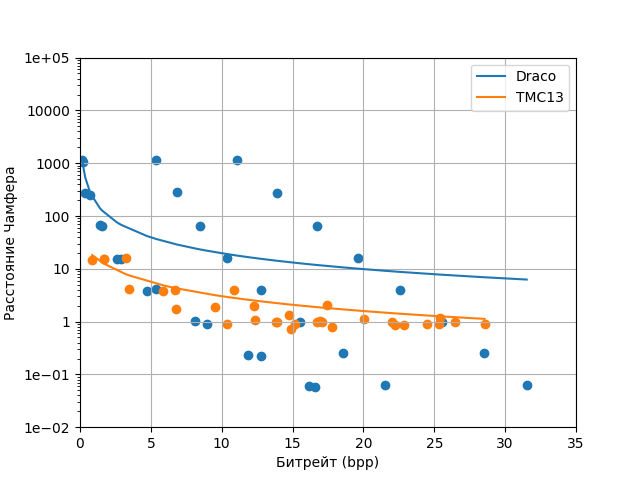
\includegraphics[width=\linewidth]{assets/pcc_arena/approx_cd_p2pt.png}
        \caption{}
    \end{subfigure}
    \begin{subfigure}{0.49\textwidth}
        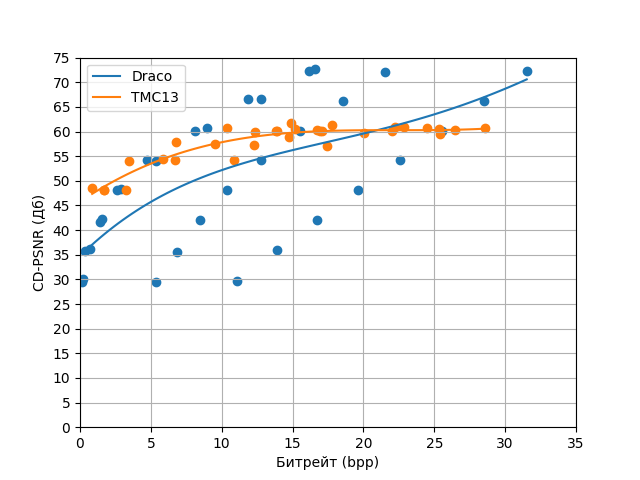
\includegraphics[width=\linewidth]{assets/pcc_arena/approx_cdpsnr_p2pt.png}
        \caption{}
    \end{subfigure}
    \caption{ (a) Зависимость расстояния Чамфера от битрейта. (b) Зависимость
    CD-PSNR от битрейта. }
    \label{img:pcc_arena_cd_bpp}
\end{figure}

На рисунке \ref{img:pcc_arena_cd_bpp} приведен график, изображающий зависимость
расстояния Чамфера от битрейта. По данному графику можно сделать вывод, что
кодек Draco показывает себя хуже относительно TMC13 при низком битрейте. При
высоком битрейте, кодеки показывают схожий результат.

\begin{figure}[H]
    \centering
    \begin{subfigure}{0.49\textwidth}
        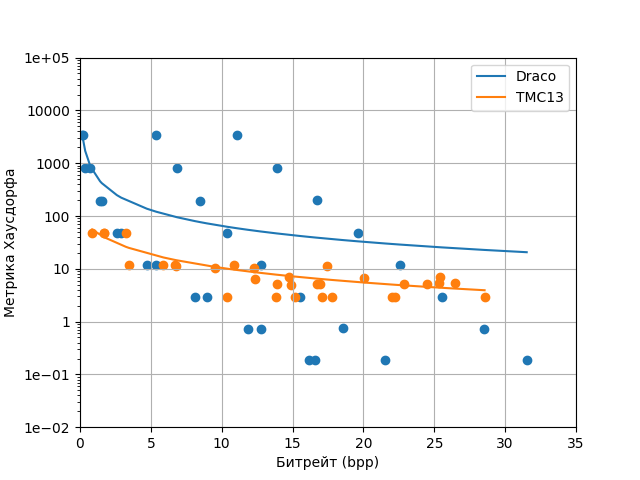
\includegraphics[width=\linewidth]{assets/pcc_arena/approx_h_p2pt.png}
        \caption{}
    \end{subfigure}
    \begin{subfigure}{0.49\textwidth}
        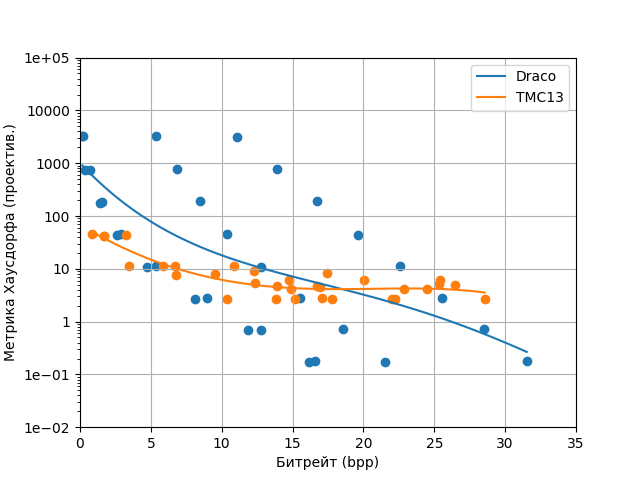
\includegraphics[width=\linewidth]{assets/pcc_arena/approx_h_p2pl.png}
        \caption{}
    \end{subfigure}
    \caption{ (a) Зависимость метрики Хаусдорфа от битрейта. (b) Зависимость
    проецированной метрики Хаусдорфа от битрейта. }
    \label{img:pcc_arena_hd}
\end{figure}

На рисунке \ref{img:pcc_arena_hd} приведен график зависимости метрики Хаусдорфа,
а также значение данной метрики при проецировании вдоль нормалей точек. Данные
графики показывают ошибку метода сжатия в худшем случае, при этом по графику
можно сделать вывод, что соотношение ошибки в худшем случае и в среднем слабо
отличается для приведенных методов сжатия. Кроме того, можно отметить, что при
проецировании ошибки вдоль нормалей, кодек TMC13 показывает незначительно
большее значение метрики Хаусдорфа, при этом значения для кодека Draco остаются
прежними, что может говорить о большем искажении нормалей кодеком TMC13.

\begin{figure}[H]
    \centering
    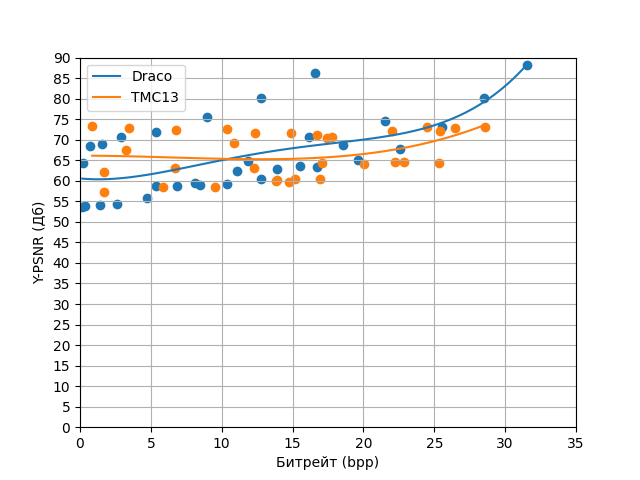
\includegraphics[width=\linewidth]{assets/pcc_arena/approx_y_psnr.png}
    \caption{ Зависимость Y-PSNR от битрейта. }
    \label{img:pcc_arena_y_psnr}
\end{figure}

На графике \ref{img:pcc_arena_y_psnr} приведено пиковое отношение сигнал-шум для
яркостной компоненты цветовой схемы Y'CbCr. По графику можно сделать вывод, что
кодек Draco сильно искажает цвета при малом битрейте, однако, при повышении
битрейта, показывает лучшие значения по сравнению с TMC13. Для TMC13 качество
передачи цвета слабо меняется в зависимости от битрейта.

% графикииии





% \chapter{Название главы}
%   \section{Названия секции}
%     \subsubsection{Название подсекции}
%       \paragraph{Название параграфа}
%         \subparagraph{Название подпараграфа}
%           \lipsum[2]\cite{BibExampleRU}
%           \begin{center}
%             \begin{xltabular}{\linewidth}{|l|X|}
%               \caption{Long table caption.\label{long}}                                                                                                    \\
%               \hline
%               Столбик1  & Столбик2    \\
%               \hline
%               слово     & Слово       \\
%               \hline
%             \end{xltabular}
%           \end{center}


% \chapter{Название главы}
%   \section{Названия секции}
%     \subsubsection{Название подсекции}
%       \paragraph{Название Параграфа}
%         \lipsum[2]\cite{BibExampleRU}
%         Как видно на \refImg{img:test} или на \refAppendix{appendix:example}
%         \fig[Длинное название картинки из примера][0.5][img:test]{assets/example.drawio.png}

%         \begin{center}
%           \begin{xltabular}{\linewidth}{|l|X|}
%             \caption{Long table caption.\label{long}}                                                                                                    \\
%             \hline
%             Столбик1  & Столбик2    \\
%             \hline
%             слово     & Слово       \\
%             \hline
%           \end{xltabular}
%         \end{center}

%         \begin{lstlisting}[caption={Название листинга}]
% begin
%   print('Hellow world!')
% end
%         \end{lstlisting}

%         \begin{itemize}
%           \item item1
%           \item item2
%         \end{itemize}

%         \begin{enumerate}
%           \item item1
%           \item item2
%         \end{enumerate}
